\documentclass[12pt,a4paper]{report}
% \usepackage[utf8]{inputenc}
% \usepackage[vietnam]{babel}
\usepackage[utf8]{vietnam}
\usepackage{amsmath}
\usepackage{amsfonts}
\usepackage{amssymb}
\usepackage{graphicx}
\usepackage{color}
\usepackage{framed}
\usepackage[left=2cm,right=2cm,top=2cm,bottom=2cm]{geometry}

\title{\framebox {
        \textcolor{TEcolor}{
            \Huge {    AP/College Physics 1    }
        }
    }    }
    
\author{\Large @arch-techs}
\date{2021}

\definecolor{TEcolor}{RGB}{0, 50, 50}

\usepackage{fancyhdr}

\pagestyle{fancy}
\fancyhf{}
\lhead{
\includegraphics[scale=0.2]{TE1}
\textcolor{TEcolor}{
\fontfamily{cmss}\selectfont
@arch-techs}
}
\rhead{\textcolor{TEcolor} {
	\fontfamily{cmss}\selectfont AP/College Physics 1
}}
\rfoot{
\fontfamily{cmss}\selectfont \textcolor{TEcolor}{
Page \thepage}}


\begin{document}
{\fontfamily{cmss}\selectfont
\begin{titlepage}
\maketitle
\end{titlepage}
\newpage

\begin{center}
    \begin{center}
    \framebox {
        \textcolor{TEcolor}{
            \Large {    AP/College Physics 1    }
        }
    }    
    \end{center}
    
    \vspace{5mm}
    
    by: @arch-techs
    
    \vspace{1cm}
    
    \begin{enumerate}
        \item Distance and displacement
            \begin{figure}[h]
                \centering
                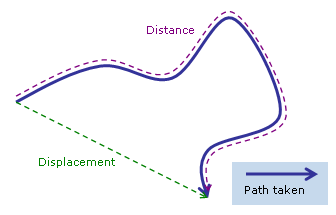
\includegraphics[scale=0.7]{Distancedisplacement}
                \fontfamily{cmss}\selectfont {
                    \caption{Distance and displacement}
                }
                \label{fig:my_label}
            \end{figure}
            \begin{itemize}
                \item Displacement: Change in position of an object. We use the symbol $\Delta x$ for displacement, where $\Delta$ means "change." A vector quantity with units of distance.
                \item Distance: Total amount the object has moved. This depends on the whole path traveled, not just the starting and ending points. Distance traveled is always a non-negative number. A scalar quantity with units of distance.
                \item Equation: \newline
                
                \begin{equation} \label{eu_eqn}
					\Delta x = x - x_{0}   		
         		\end{equation}
				\begin{center}
				$\Delta x$ is displacement, $x$ is the final position, $x_{0}$ is the initial position.
				\\
				Displacement is the difference between the final and initial positions.
				\end{center}				         		
         		
                
            \end{itemize}
            
   		\item Average velocity and speed
   			\begin{align*}
   				\overline{v} = \dfrac{\Delta x}{\Delta t} && / && v_{arg} = \dfrac{d}{\Delta t}
   			\end{align*}
   		
               
        \newpage

   		
            
    \end{enumerate}

    
    \begin{enumerate}
        \item Chuyển động thẳng đều và những đại lượng đặc trưng:
            \begin{enumerate}
                \item Vận tốc, gia tốc và phương trình chuyển động:
                    \[\left\{
                    \begin{array}{lr}
                    x.v = const \\
                    a = 0  \\
                    s = v.t \\
                    \end{array}
                    \right.
                    \]
                    \[\Rightarrow x = v.t\]
            \end{enumerate}
        \item Chuyển động thẳng biến đổi đều:
            \begin{enumerate}
                \item Vận tốc và gia tốc: \[
                    \left\{
                    \begin{array}{lr}
                    v = v_{0} + a.t \\
                    a = const
                    \end{array}
                    \right.
                \]
                \item Phương trình chuyển động: \[
                    s = v_{0}.t + \dfrac{1}{2}.a.t^{2}  \rightarrow  x = x_{0} + v_{0}.t + \dfrac{1}{2}.a.t^{2}
                \]
                \item Hệ thức liên hệ: \[
                    v^{2} - v_{0}^{2} = 2.a.s  
                \]
            \end{enumerate}
        \item  Chuyển động tròn:
            \begin{enumerate}
                \item Gia tốc hướng tâm và gia tốc tiếp tuyến:\[
                    \left\{
                    \begin{array}{lr}
                        a_{n} = \dfrac{d^{2}}{r} = \omega ^{2}.r \\
                        a_{t} = \beta r & :  \beta = const
                    \end{array}
                    \right.  
                \]
                \item Gia tốc toàn phần: \[a = \sqrt{a_{n}^{2} + a_{t}^{2}} = r\sqrt{\omega ^{4} + \beta ^{2}}\]
                \item Một số công thức liên hệ: \[v = \omega r ; \quad T = \dfrac{2\pi}{\omega}\]
                \item Phương trình chuyển động: \[
                    \left\{
                    \begin{array}{lr}
                        \omega_{t} = \omega_{0} + \beta .t \\
                        \varphi_{t} = \varphi_{0} + \omega_{0}t + \dfrac{1}{2} \beta t^{2} \\
                        \beta = const
                    \end{array}
                    \right.  
                \]
                \item Trường hợp chuyển động tròn đều: \[
                    \left\{
                    \begin{array}{lr}
                        \omega = const \\
                        \varphi = \varphi_{0} + \omega_{0} t     
                    \end{array}
                    \right.
                \]
            \end{enumerate}

            \item Chuyển động rơi tự do:
            \begin{enumerate}
                \item Vận tốc và quãng đường chuyển động: \[
                    \left\{
                    \begin{array}{lr}
                    v = v_{0} + g.t \\
                    s = v_{0}.t + \dfrac{1}{2}gt^{2} 2       
                    \end{array}
                    \right.
                    \]
                    \[\rightarrow v^{2} - v_{0}^{2} = 2gs = 2gh\]
                \newpage
                \item Thời gian rơi từ độ cao h cho đến khi chạm đất:
                \[t = \sqrt{\dfrac{2h}{g}}\]
            \end{enumerate}
            \item  Chuyển động ném xiên:
            \begin{enumerate}
                \item Quỹ đạo là nhanh parabol
                \[ y = -\dfrac{g}{2v_{0}^{2} {\cos ^{2} \alpha}} x^{2} + x \tan \alpha\]
                \item Tầm ném xa: 
                \[L = \dfrac{v_{0}^{2} \sin 2\alpha}{g}  \rightarrow L_{max} = \dfrac{v_{0}^{2}}{g} : \alpha = 45^{0}\]    
                \item Độ cao cực đại:
                \[h_{max} = \]
            \end{enumerate}

    \end{enumerate}

\end{center}




}
\end{document}